%\renewcommand{\theequation}{\theenumi}
%\begin{enumerate}[label=\arabic*.,ref=\thesubsection.\theenumi]
%\numberwithin{equation}{enumi}
%
% 
Let 
\begin{align}
\vec{x} = \myvec{a\\0}
\end{align}
%
Substituting in \eqref{eq:1.2.1_p1}, 
%
\begin{align}
\myvec{1 & -1} \myvec{a\\0}&= -1
\\
\implies a &=-1
\end{align}
%
Simiarly, substituting 
%
\begin{align}
\vec{x} &= \myvec{0\\b},
\end{align}
%
in \eqref{eq:1.2.1_p1}, 
%
%
\begin{align}
b =1
\end{align}
%
The intercepts on the x and y-axis from above are 
\begin{align}
%\vec{A} = 
\myvec{-1\\0}, 
%\vec{B} = 
\myvec{0\\1}
\end{align}
%The python code for the Problem \eqref{eq:1.2.1_p1}
%%
%can be used to plot Fig. \ref{fig:1.2.1_intercept1}.
%%
%\begin{figure}[!ht]
%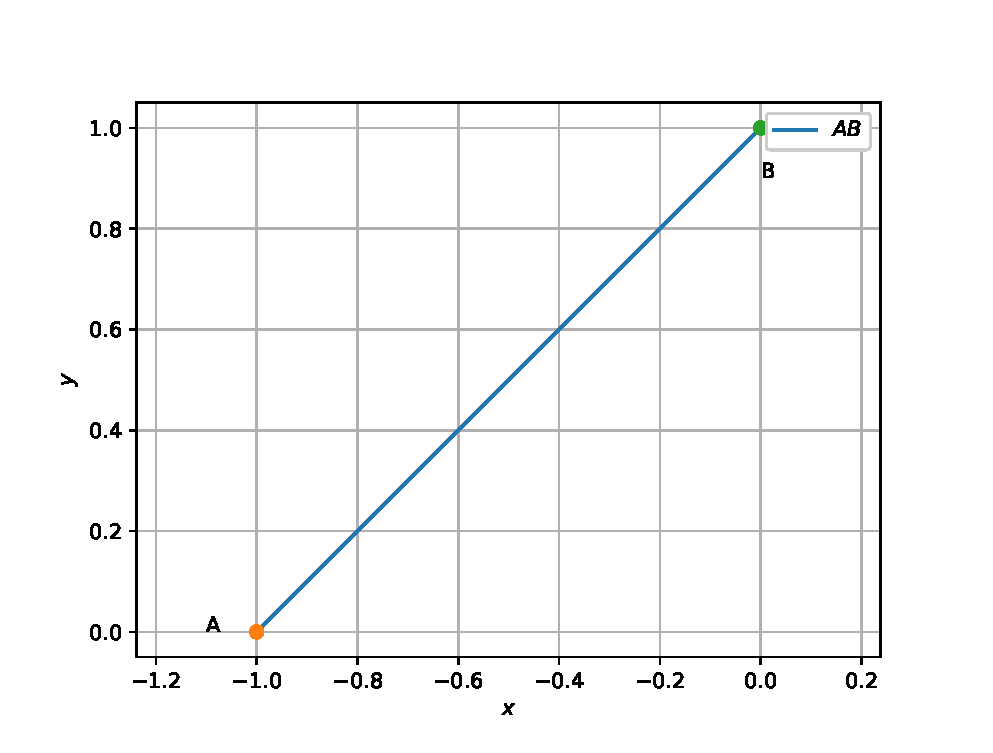
\includegraphics[width=\columnwidth]{./solutions/1/figs/triangle/icept1.eps}
%\caption{Intercept 1}
%\label{fig:1.2.1_intercept1}
%\end{figure}
%
%\label{eq:1.2.1_p1xaxis}
%$\vec{A}$ is the x-intercept of the line and is the point where it meets x-axis.
%\\
Similarly, the intercepts on x and y-axis for \eqref{eq:1.2.1_p2} are
\begin{align}
\myvec{4\\0}, 
\myvec{0\\6}
\end{align}

%\label{eq:1.2.1_p2xaxis}
%$\vec{C}$ is the x-intercept of the line and is the point where it meets x-axis.
%The python code for the Problem \eqref{eq:1.2.1_p2}
%%
%can be used to plot Fig. \ref{fig:1.2.1_intercept2}.
%%
%\begin{figure}[!ht]
%\includegraphics[width=\columnwidth]{./solutions/1/figs/triangle/icept2.eps}
%\caption{Intercept 2}
%\label{fig:1.2.1_intercept2}
%\end{figure}
%
The interection of the lines in \eqref{eq:1.2.1_p1}, \eqref{eq:1.2.1_p1}
is obtained  from
\begin{align}
\myvec{1 & -1\\3 & 2} \vec{x} = \myvec{-1\\12}
\end{align}
%
The augmented matrix for the above equation is row reduced as follows
\begin{align}
\myvec{1 & -1 & -1\\3 & 2 & 12} 
\xleftrightarrow {R_2\leftarrow \frac{R_2-3R_1}{5}}\myvec{1 & -1 & -1\\0 & 1 & 3} 
\\
%\myvec{1 & -1 & -1\\0 & 1 & 3} 
\xleftrightarrow {R_1\leftarrow R_1 + R_2}\myvec{1 & 0 & 2\\0 & 1 & 3} 
\label{eq:1.2.1_line_aug}
\end{align}
%
\begin{align}
\implies \vec{x}=\myvec{2\\3}
\end{align}
%The equivalent python code is
%%
%\begin{lstlisting}
%codes/triangle/line_intersect.py
%\end{lstlisting}
%%
%which plots Fig. \ref{fig:1.2.1_line_intercept}, intersect at $\myvec{2\\3}$
%%
%\begin{figure}[!ht]
%\includegraphics[width=\columnwidth]{./solutions/1/figs/triangle/line_intercept.eps}
%\caption{Line intercept}
%\label{fig:1.2.1_line_intercept}
%\end{figure}

The desired triangle is available in Fig.  \eqref{fig:1.2.1_Shaded} with vertices
\begin{align}
\vec{A}=\myvec{2\\3},
%\\
\vec{B}=\myvec{-1\\0},
%\\
\vec{C}=\myvec{4\\0}
\end{align}
\begin{figure}[!ht]
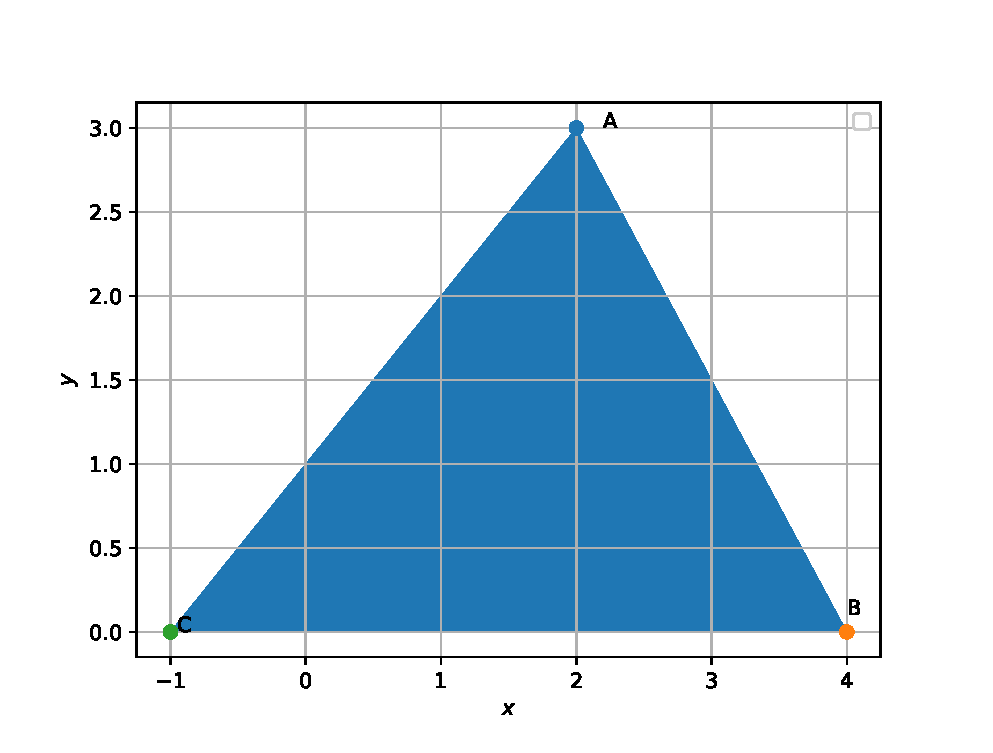
\includegraphics[width=\columnwidth]{./solutions/1/figs/triangle/shaded.eps}
\caption{}
\label{fig:1.2.1_Shaded}
\end{figure}
The equivalent python code for figure \eqref{fig:1.2.1_Shaded} is
%
\begin{lstlisting}
solutions/1/codes/triangle/shaded.py
\end{lstlisting}

